%!TEX root = main.tex

\newpage
\section{문서 작성 시작하기}
\label{sec:text}
\subsection{예시 코드 구경하기}
그럼 지금부터는 본격적으로 문서 작성을 시작해 보도록 하겠습니다.
사실 진짜 기본적인 내용은 \ref{sec:beginning}에서 모두 끝났기 때문에, 지금부터는 \lt 의 각 기능들을 어떻게 활용하는지에 초점을 맞추어 살펴보도록 하겠습니다. 아마 여기도 예시를 들어 설명하는 것이 보다 이해가 쉬울 겁니다. 간단한 예시 코드를 보도록 하죠.
\begin{Verbatim}[frame=single]
\documentclass{article}
\usepackage{kotex}
\usepackage[left=2.5cm,right=2.5cm,top=3cm,bottom=3cm,a4paper]{geometry}
\author{KSAstudent}
\date{\today}
\title{이게 레이텍입니다}
\begin{document}
    \maketitle
    \tableofcontents
    \vspace{3cm}
    \section{글 작성하기}
    \label{sec:intro}

        \subsection{기본적인 글}
        \label{sec:text}
        그냥 적으면 됩니다. ㅎㅎ
        
        \subsection{그림 넣기}
        \label{sec:image}
        \begin{center}
          \emph{뒤에서} 설명드릴게요.
        \end{center}

    \section{수식 작성하기}
    \ref{sec:image}와 크게 다르지 않습니다.\\
    뒤에서 설명드릴게요.

\end{document}
\end{Verbatim}
이 코드의 결과물은 다음 페이지에서 확인하실 수 있습니다.

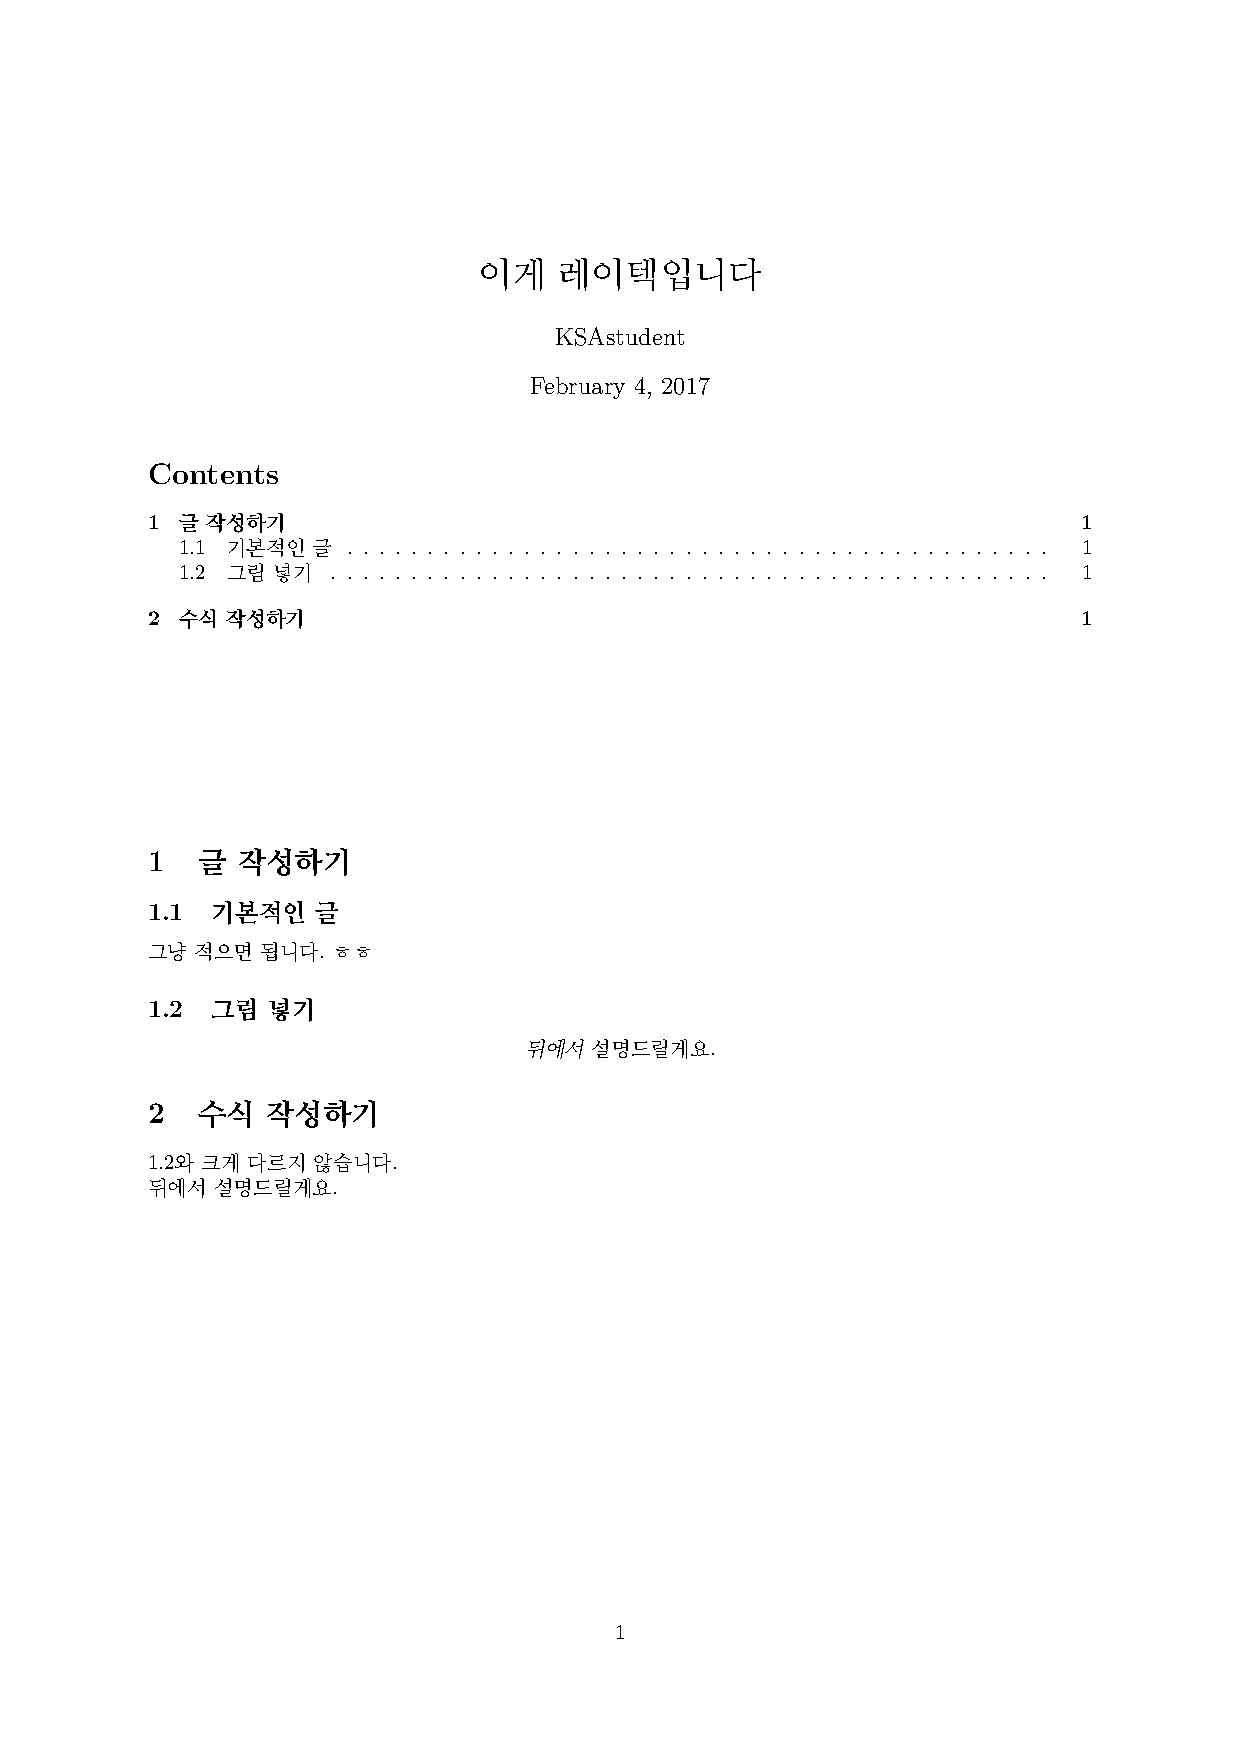
\includepdf[fitpaper=true]{example/examplepdf.pdf}

이해하셨나요? 지금부터 천천히 하나씩 살펴봅시다.

\subsection{글의 구조}
\label{sec:text-org}
일단 글의 전체적인 구조부터 파악해 봅시다.
앞서 \ref{preamble}에서 preamble에 대한 설명을 들으셨을 겁니다.
\verb|\documentclass| 부터 \verb|\begin{document}| 까지가 preamble에 속합니다.
그 아래 \verb|\begin{document}|부터 \verb|\end{document}|까지는 글의 실질적인 내용에 속하죠.

글의 내용을 천천히 살펴봅시다.
여기서 사용된 article 이라는 class는 section부터 시작해 subsection, subsubsection, paragraph 순으로 이어지는 문서 구조를 가지고 있습니다.
첫 번째 section의 첫 번째 subsection은 1.1, 두 번째 subsection은 1.2, ... 이런 식으로 구조화가 이루어지는 거죠.
앞서 말씀드렸듯이 \verb|\begin{}|과 \verb|\end{}|는 다양한 용도로 사용됩니다.
\verb|\begin{}|과 \verb|\end{}|사이를 하나의 환경, envorinment라고 부르는데, 여기서는 center라는 envorinment를 정의하기 위해 사용되었죠.
특정 environment안의 글들은 그 environment의 특징을 띄게 됩니다.
여기서 center라는 environment는 글을 가운데 정렬하는 역할을 합니다.

거의 대부분의 \lt 코드들은 본질적으로  위 코드와 크게 다르지 않습니다.
environment안에 environment가 있다거나 하는 복잡한 구조라도, 펼쳐놓고 보시면 이걸로도 충분히 이해하실 수 있습니다.

\subsection{Preamble의 기능}
\label{sec:text-preamble}
그렇다면 지금부터는 아까 설명드린 preamble 각 줄이 어떤 역할을 하는지 보다 구체적으로 살펴보도록 하겠습니다.
사실 제가 예시로 든 것 말고도 수많은 package나 기능들이 있지만, 일단 그것들이 어떤 식으로 사용되는지 이해해 보시라는 의미에서 몇 가지 자주 쓰일만한 것들만 예시로 넣었습니다.
\begin{itemize}
  \item 우선 맨 첫줄의 \verb|\documentclass|에 대한 설명은 \ref{documentclass}에서 충분히 했으니 다음 줄부터 설명하겠습니다. 다양한 document class들은 나중에 하나씩 살펴보도록 하고요.

  \item \verb|\usepackage{kotex}|는 \ref{sec2-package}에서 잠깐 언급했지만, 한글을 사용하기 위해 사용되는 package입니다. 이 package 없이는 한글이 제대로 표시되지 않죠.

  \item 다음 줄의 \verb|\usepackage[...]{geometry}| 부분을 살펴보도록 하겠습니다. \verb|\usepackage{geometry}|는 geometry라는 이름의 package를 사용하겠다는 명령이고, 사이에 있는 대괄호는 그 geometry라는 package를 어떻게 사용할 것인지, 옵션을 지정하는 부분입니다. Geometry라는 이름에서, 그리고 옵션의 내용에서 짐작하실 수 있듯이 이 package는 문서의 여백을 설정할 수 있는 package입니다. 사실 굳이 지정을 안하셔도 \lt 는 기본 설정대로 예쁜 문서를 만들어 줍니다. 그렇지만 문제가 있다면 여백이 조금 넓다는 거죠. 직접 한 번 해 보시면 아실 겁니다. 사실 이 여백은 어떻게 하면 가장 읽기 편한 문서를 만들 수 있을지, 다양한 방면에서 고려해 결정된 것이라곤 합니다. 그렇기에 저도 저 혼자 볼 문서는 기본 설정대로 만드는 경우가 많고요. 그렇지만 솔직히 여백이 너무 넓으면 부담스러운 경우가 많지 않습니까. 그럴 땐 이 패키지를 쓰시면 됩니다.
    
  \item 다음 세 줄은 연달아 author, date, title을 지정했네요. 별 거 없습니다. 말 그대로 지정한 거죠. 몇 줄 내려가 \verb|\begin{document}|아래에 \verb|\maketitle|이 보이시나요? 거기서는 여기서 지정한 값들을 바탕으로 제목을 만들어 줍니다. 아, \verb|\today|는 뭐냐고요? date 자리에 오늘 날짜를 자동으로 입력해 주는 명령어입니다. 굳이 \verb|\today|를 쓰지 않고 그냥 아무거나 넣으면 날짜 자리에 그게 뜰겁니다. 
\end{itemize}

이 코드의 preamble은 이게 전부입니다. 간단하죠?
이 코드에서 사용된 것 말고도  preamble에서는 다양한 일을 할 수 있습니다.
앞서 \ref{sec:1.2-ext}에서 잠깐 언급했지만 새로운 명령을 정의해서 사용한다거나, 명령들이 어떻게 작동할지 구체적으로 설정하는 것도 가능합니다.
몇 가지는 뒤에서 천천히 소개하겠습니다.


\subsection{명령어 알아보기}
\label{sec:3-cmd}
지금부터는 \lt 의 명령어들을 구체적으로 알아보겠습니다.
사실 명령어라고 거창하게 이름 붙일 것도 없습니다.
앞에서 눈치채셨겠지만 \lt 는 \verb|\|로 시작하는 단어를 인식하고, 이는 모두 명령어라고 불리기 때문입니다.

%%% Local Variables:
%%% mode: latex
%%% TeX-master: "main"
%%% End:
